\documentclass[12pt,a4paper]{article}

% ── Encodage & langue ──────────────────────────────────────────────────────────
\usepackage[utf8]{inputenc}
\usepackage[T1]{fontenc}
\usepackage[french]{babel}

% ── Mise en page ───────────────────────────────────────────────────────────────
\usepackage[top=2.5cm, bottom=2.5cm, left=2.5cm, right=2.5cm]{geometry}
\usepackage{parskip}
\usepackage{setspace}
\onehalfspacing

% ── Typographie ────────────────────────────────────────────────────────────────
\usepackage{lmodern}
\usepackage{microtype}

% ── Mathématiques ──────────────────────────────────────────────────────────────
\usepackage{amsmath, amssymb}

% ── Tableaux ───────────────────────────────────────────────────────────────────
\usepackage{booktabs}
\usepackage{tabularx}
\usepackage{array}
\usepackage{multirow}
\usepackage{longtable}

% Graphics
\usepackage{graphicx}
\graphicspath{{../img/}{img/}{./img/}}

% ── Code source ────────────────────────────────────────────────────────────────
\usepackage{listings}
\usepackage{xcolor}

\definecolor{codebg}{RGB}{245,245,245}
\definecolor{codeframe}{RGB}{200,200,200}
\definecolor{codecomment}{RGB}{100,100,100}
\definecolor{codestring}{RGB}{163,21,21}
\definecolor{codekeyword}{RGB}{0,0,255}

\lstset{
  backgroundcolor=\color{codebg},
  frame=single,
  rulecolor=\color{codeframe},
  basicstyle=\ttfamily\small,
  keywordstyle=\color{codekeyword}\bfseries,
  stringstyle=\color{codestring},
  commentstyle=\color{codecomment}\itshape,
  breaklines=true,
  showstringspaces=false,
  language=Python,
  literate=
    {é}{{\'{e}}}1 {è}{{\`{e}}}1 {ê}{{\^{e}}}1 {ë}{{\"e}}1
    {à}{{\`{a}}}1 {â}{{\^{a}}}1 {î}{{\^{i}}}1 {ô}{{\^{o}}}1
    {û}{{\^{u}}}1 {ù}{{\`{u}}}1 {ç}{{\c{c}}}1 {œ}{{\oe}}1
}

% ── Hyperliens ─────────────────────────────────────────────────────────────────
\usepackage[colorlinks=true, linkcolor=blue!70!black, urlcolor=blue!70!black]{hyperref}

% ── En-têtes / pieds de page ───────────────────────────────────────────────────
\usepackage{fancyhdr}
\setlength{\headheight}{14.2pt}
\addtolength{\topmargin}{-2.2pt}
\pagestyle{fancy}
\fancyhf{}
\lhead{\small Analyse de conversations patient-thérapeute - Étape 1}
\rhead{\small LARROUX Logan}
\cfoot{\thepage}
\renewcommand{\headrulewidth}{0.4pt}

% ══════════════════════════════════════════════════════════════════════════════
\begin{document}

% ── Page de titre ──────────────────────────────────────────────────────────────
\begin{titlepage}
  \centering
  \vspace*{2cm}
  {\LARGE\bfseries Analyse de conversations patient-thérapeute\\[0.4em]
  sur la santé mentale\par}
  \vspace{1.5cm}
  {\large Étape 1 — Exploration du jeu de données\par}
  \vspace{2cm}
  {\large\bfseries LARROUX Logan\par}
  {\normalsize Étudiant en licence Informatique — Université de Toulouse\par}
  \vspace{1cm}
  {\normalsize Encadrante : Lynda Tamine-Lechani\par}
  \vspace{0.5cm}
  {\normalsize Projet [Info5.BE-SHS] — 2025/2026\par}
  \vfill
  {\small Données : \href{https://www.kaggle.com/datasets/thedevastator/nlp-mental-health-conversations}{Kaggle — NLP Mental Health Conversations}\par}
  {\small Code : \href{https://github.com/cypnet/Analyse-de-conversations-sur-la-sant-mentale/tree/main/notebooks/LOGAN}{GitHub — branche Logan}\par}
\end{titlepage}

% ── Table des matières ─────────────────────────────────────────────────────────
\tableofcontents
\newpage

% ══════════════════════════════════════════════════════════════════════════════
\section{Introduction}

La santé mentale est un enjeu majeur de la santé publique. Ce projet vise, dans un premier
temps, à exploiter le jeu de données pour comprendre les types de conversations et leur
structure, puis à analyser les sentiments des échanges afin de détecter les émotions et états
psychologiques des patients. Ensuite, il se concentre sur l'accès et le traitement des
conversations, en résumant les échanges et en identifiant les schémas linguistiques récurrents.
Enfin, il prévoit le développement d'un système question-réponse, capable d'automatiser les
interactions et fournir des réponses.

Le jeu de données utilisé est composé de deux colonnes : \texttt{Context} (messages du patient)
et \texttt{Response} (réponses du thérapeute).

% ══════════════════════════════════════════════════════════════════════════════
\section{Pré-traitement des données}

\subsection{Nettoyage}

Avant toute analyse, plusieurs étapes de nettoyage ont été appliquées dans l'ordre suivant.

\textbf{Suppression des cellules vides et des doublons.}
Les lignes contenant des valeurs nulles dans les colonnes \texttt{Context} ou \texttt{Response}
ont été supprimées, ainsi que les lignes entièrement dupliquées.

\textbf{Filtrage des textes non-anglais.}
Le corpus contenait des phrases en espagnol. La bibliothèque \texttt{langdetect} a été utilisée
pour détecter la langue de chaque ligne et ne conserver que les textes identifiés comme anglais.
Cette détection est effectuée au niveau de la phrase entière, ce qui est bien plus fiable qu'une
détection mot par mot.

\begin{lstlisting}
from langdetect import detect, LangDetectException

def is_english_text(text):
    try:
        return detect(str(text)) == 'en'
    except LangDetectException:
        return True  # texte trop court -> on garde

mask = df['Context'].apply(is_english_text) \
     & df['Response'].apply(is_english_text)
df = df[mask].reset_index(drop=True)
\end{lstlisting}

\textbf{Normalisation.}
Tous les textes ont été passés en minuscules afin d'éviter que \textit{"Toto"} et \textit{"toto"}
soient traités comme deux mots distincts. Les espaces insécables (\texttt{\textbackslash xa0}),
fréquents dans des données extraites du web, ont également été supprimés.

\subsection{Tokenisation}

La tokenisation consiste à découper chaque phrase en unités élémentaires appelées
\textit{tokens}. La bibliothèque \textbf{spaCy} (\texttt{en\_core\_web\_sm}) a été utilisée
pour cette étape, via \texttt{nlp.pipe()} afin de traiter les données en batch et réduire le
temps de traitement.

\subsection{Suppression de la ponctuation et des mots vides}
\label{stopwords}

Les \textit{stopwords} (mots vides) sont des mots sans réelle signification sémantique
(pronoms, adverbes, mots de liaison). spaCy les identifie automatiquement via l'attribut
\texttt{token.is\_stop}. Les tokens de ponctuation ont été supprimés de la même façon avec
\texttt{token.is\_punct}.

Des mots trop génériques mais non reconnus comme stopwords ont également été filtrés
manuellement :

\begin{lstlisting}
extra_stopwords = {
    "feel", "like", "want", "know", "time",
    "thing", "good", "need", "year", "think",
    "tell", "say", "come", "go"
}
\end{lstlisting}

\subsection{Lemmatisation}

La lemmatisation transforme chaque mot en sa forme de base (\textit{"running"} $\rightarrow$
\textit{"run"}, \textit{"better"} $\rightarrow$ \textit{"good"}). Cette étape réduit
drastiquement le nombre de tokens distincts et regroupe les formes similaires. Elle a également
permis de filtrer les URLs, emails et chiffres dans une seule passe :

\begin{lstlisting}
df["Context_clean"] = [
    [
        token.lemma_
        for token in doc
        if not token.is_stop
        and not token.is_punct
        and not token.is_space
        and not token.like_num
        and not token.like_url
        and not token.like_email
        and token.is_alpha
        and token.lemma_ not in extra_stopwords
    ]
    for doc in docs_context
]
\end{lstlisting}

\textit{Note : spaCy lemmatise différemment selon le contexte grammatical. Par exemple,
\textit{"feeling"} utilisé comme nom reste tel quel au lieu d'être ramené à \textit{"feel"}.
C'est pourquoi \textit{"feel"} a été retiré manuellement des extra\_stopwords pour éviter
les doublons sémantiques.}

% ══════════════════════════════════════════════════════════════════════════════
\section{Analyse statistique}
\label{sec:analyse_statistique}

\subsection{Nombre de patients et thérapeutes uniques}
\label{sec:nbPatientsTherapeutes}

Il n'existe pas vraiment de façon assez fiable pour différencier un patient/thérapeute d'un autre, 
la solution aurait été d'avoir un identifiant unique pour chaque patient/thérapeutes.
En l'absence de cela dans le dataset, le nombre de patients uniques est estimé
par le nombre de valeurs distinctes dans la colonne \texttt{Context}, et de même pour les
thérapeutes avec \texttt{Response}. Cette méthode reste approximative.

\subsection{Nombre de mots moyens par conversation}

Le tableau suivant compare la longueur moyenne des messages avant et après lemmatisation :

\begin{table}[h]
\centering
\begin{tabularx}{0.60\textwidth}{lXX}
\toprule
\textbf{Mesure} & \textbf{Patients} & \textbf{Thérapeutes} \\
\midrule
Avant nettoyage      & 820 & 819 \\
Après nettoyage      & 2405 & 1985 \\
\bottomrule
\end{tabularx}
\caption{Longueur moyenne des messages avant et après nettoyage}
\end{table}

\subsection{Distribution des conversations par thérapeutes}

On cherche ici combien de conversations peut avoir un thérapeutes avec un ou plusieurs patients. 
Or le problème ici est que, comme mentionné précedemment (section \ref{sec:nbPatientsTherapeutes}), 
il n'existe pas de moyen fiable pour différencier les patients et les thérapeutes, et donc aucuns moyens de déterminer le nombre de conversations par thérapeutes.

\pagebreak

\subsection{Nombre d'échanges moyen par conversations}
En supposant que tout les patients et thérapeutes sont uniques, on va chercher le nombre de \textbf{mot moyens par patients/thérapeutes} sous plusieurs conditions:
avec les \textit{stopwords}, sans les \textit{stopwords} et avec la lemmatisation.

\begin{table}[h]
\centering
\begin{tabularx}{0.60\textwidth}{lXX}
\toprule
\textbf{Mesure} & \textbf{Patients} & \textbf{Thérapeutes} \\
\midrule
Avec \textit{stopwords}     & 290.77 & 1011.24 \\
Sans \textit{stopwords}     & 26.55 & 87.95 \\
Après lemmatisation         & 16.29 & 59.69 \\
\bottomrule
\end{tabularx}
\caption{Nombre de mots moyens par patients/thérapeutes selon les différentes étapes de nettoyage}
\end{table}

On peut donc constater que: \\
\begin{itemize}
  \item \textbf{avec les stopwords}, les thérapeutes utilisent plus de mots que les patients (\textbf{28.75\% de plus}).
  \item \textbf{après lemmatisation}, les thérapeutes utilisent plus de mots que les patients (\textbf{27.29\% de plus}).
\end{itemize}

\vspace{0.5cm}

\begin{figure}[h]
\centering
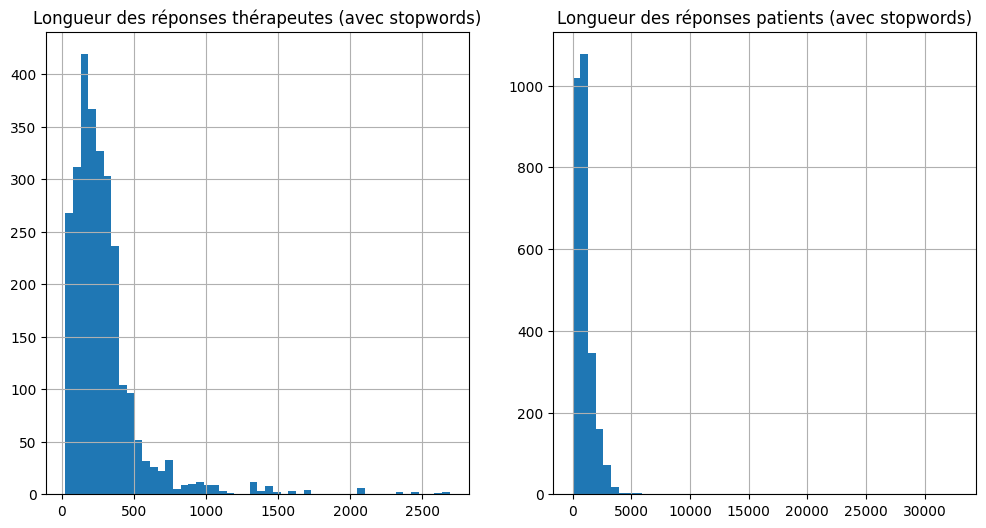
\includegraphics[width=0.45\textwidth]{graph_longRep_avec_stopwords.png}
\hfill
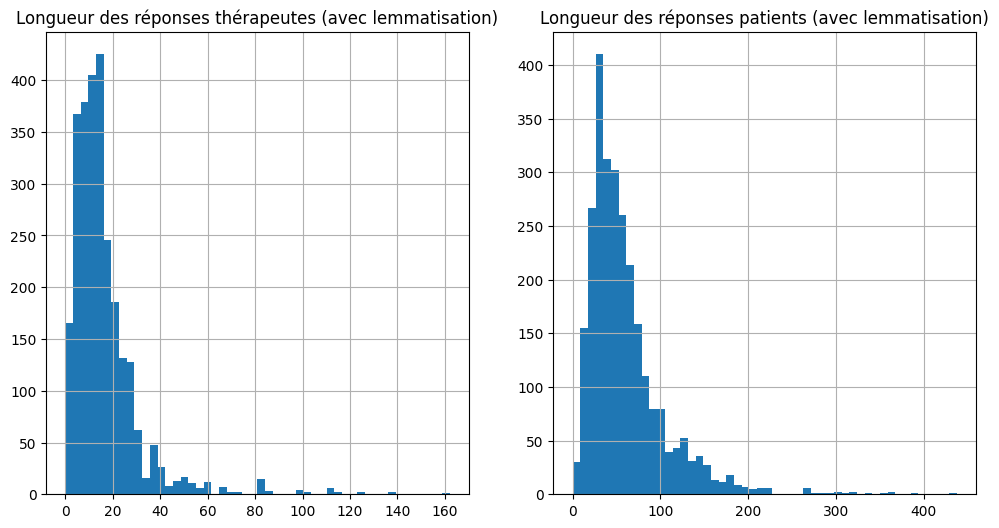
\includegraphics[width=0.45\textwidth]{graph_longRep_lemma.png}
\caption{Distribution des longueurs des messages des thérapeutes avant et après lemmatisation}
\end{figure}

\pagebreak

\subsection{Mots les plus fréquents}
En précisant que l'on a retiré des stopwords supplémentaires (mentionnée dans la section \ref{stopwords}),
on peut constater que les mots les plus fréquents sont des termes génériques liés à la santé mentale, tels que
\textit{"anxiety"}, \textit{"depression"}, \textit{"help"}, \textit{"family"}, \textit{"relationship"}, etc. 
Ces mots reflètent les thèmes centraux abordés dans les conversations, une information supplémentaire qui nous sera utile
dans les modèles.

\begin{figure}[h]
\centering
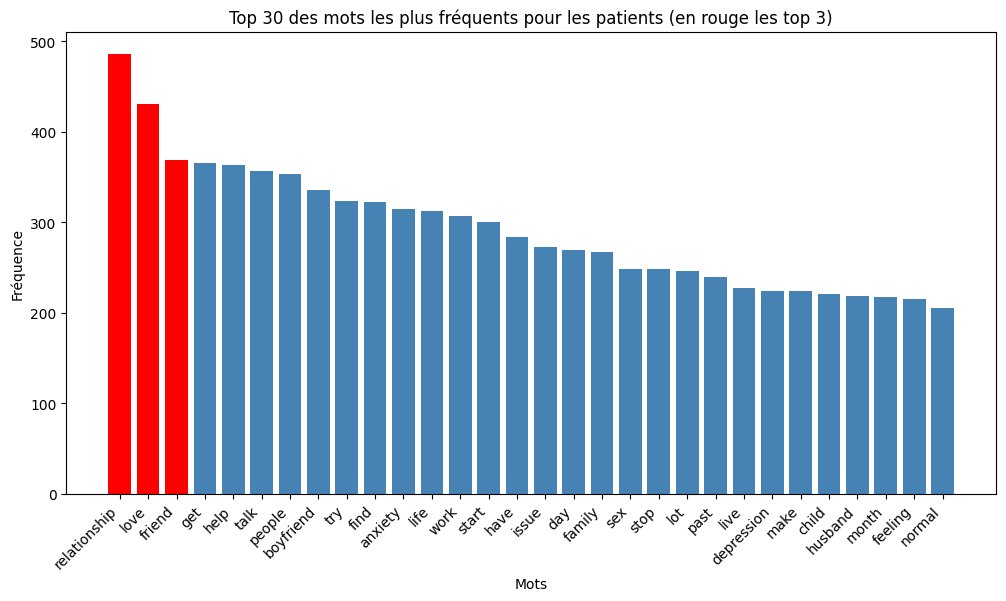
\includegraphics[width=0.45\textwidth]{hist_mot_frequent_patient.png}
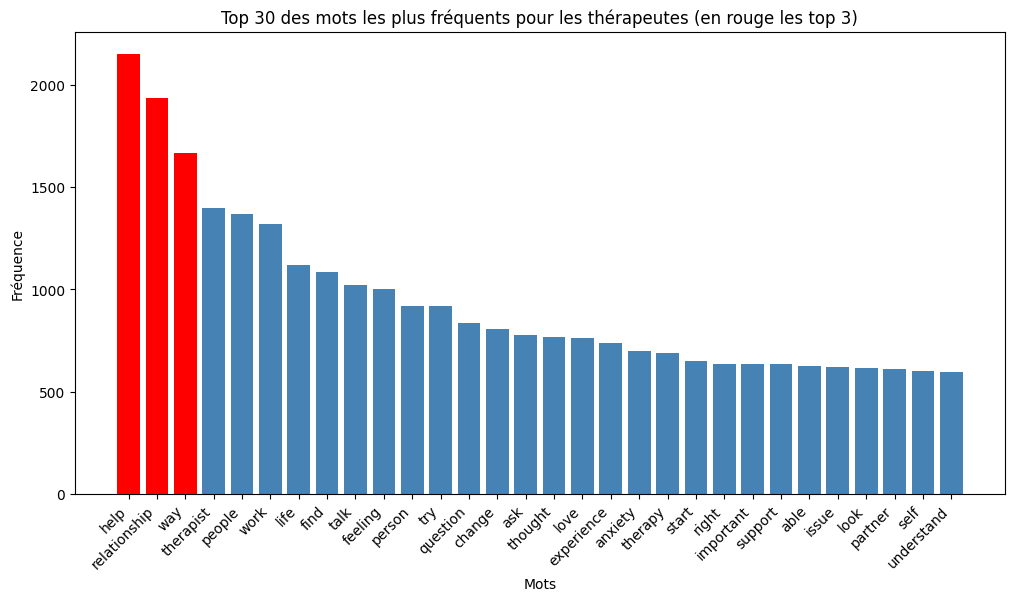
\includegraphics[width=0.45\textwidth]{hist_mot_frequent_therapeute.png}
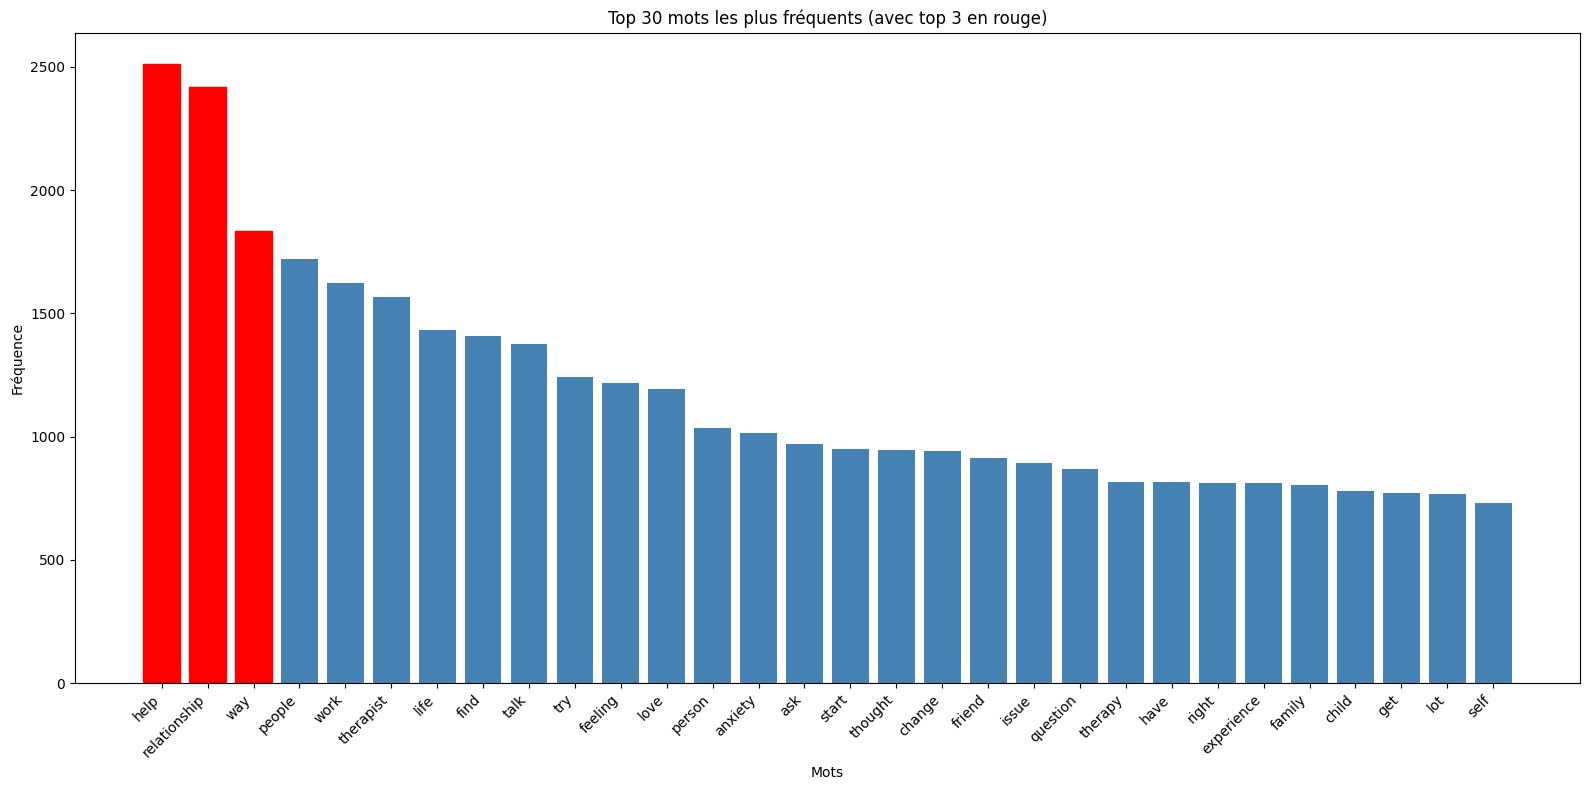
\includegraphics[width=0.70\textwidth]{hist_mot_frequent_global.png}
\caption{Mots les plus fréquents chez les patients/thérapeutes et globalement}

\end{figure}

Si on aurait gardé \textit{feel} des mots à analyser, on aurait remarqué ici que \textit{feel} 
et \textit{feeling} sont deux termes distincts, alors que leur sens est très proche. 
Cela vient du fait que spaCy \textbf{lemmatise différement selon le contexte grammatical} du mot.
Quand feeling est utilisé comme nom (\textit{"a feeling of anxiety"}), spaCy le garde tel quel au lieu de le remener à \text{feel}.\\
Ensuite, \textit{like} est un mot ambigue en anglais, il peut être un verbe (\textit{"I like this"}) ou une préposition (\textit{"feel like crying"}), 
auquel cas c'est quasiment un mot vide d'où sa suppression. 

\pagebreak

\subsection{Corrélation patient / thérapeute}

La correlation mesure, dans notre cas, le lien qu'il peut y avoir entre la longueur des phrases du patient et du thérapeute.
Cela nous permet de voir si les thérapeutes adaptent la longueur de leurs réponses à celle des messages des patients, 
ou si au contraire ils utilisent des réponses de longueur relativement constante indépendamment de la longueur du message patient.

Le résultat obtenu est une \textbf{corrélation proche de 0} ($\approx 0.05$), 
cela signifie qu'\textbf{un patient peut s'exprimer longuement et recevoir une réponse courte, et
inversement}. Les réponses des thérapeutes semblent donc relativement indépendantes de la
longueur des messages patients, ce qui peut s'expliquer par l'utilisation de réponses
standardisées ou formulées de façon uniforme.

\begin{figure}[h]
\centering
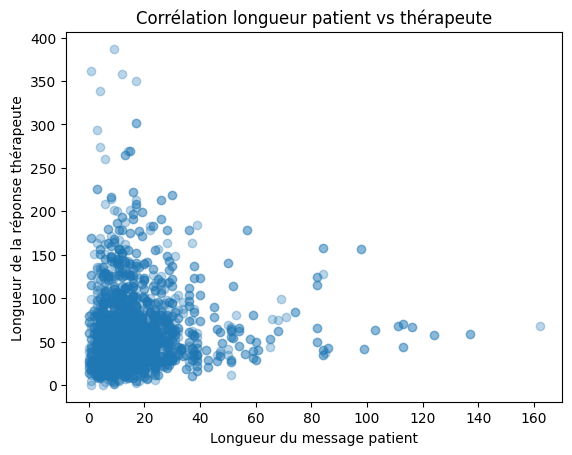
\includegraphics[width=0.6\textwidth]{plot_correlation_patient_therapeute.png}
\caption{Nuage de points représentant la longueur des messages patients (en abscisse) et thérapeutes (en ordonnée)}
\end{figure}

\pagebreak

\subsection{Hapax legomena}

Un \textit{hapax} est un mot qui n'apparaît qu'\textbf{une seule fois dans le corpus}. L'analyse des
mots les moins fréquents a révélé que la plupart des hapax sont du \textbf{bruit résiduel} (abréviations,
artefacts de nettoyage ou même mot en espagnol passé à travers les mailles du fillet), 
ce qui confirme l'importance du filtrage préalable.

\begin{figure}[h]
\centering
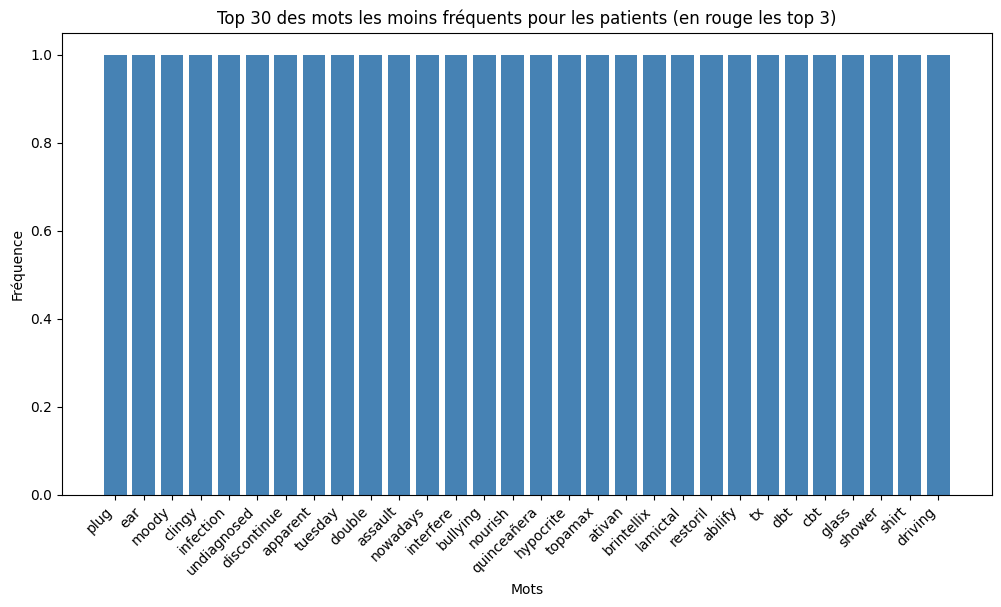
\includegraphics[width=0.80\textwidth]{hist_hapax_patient.png}
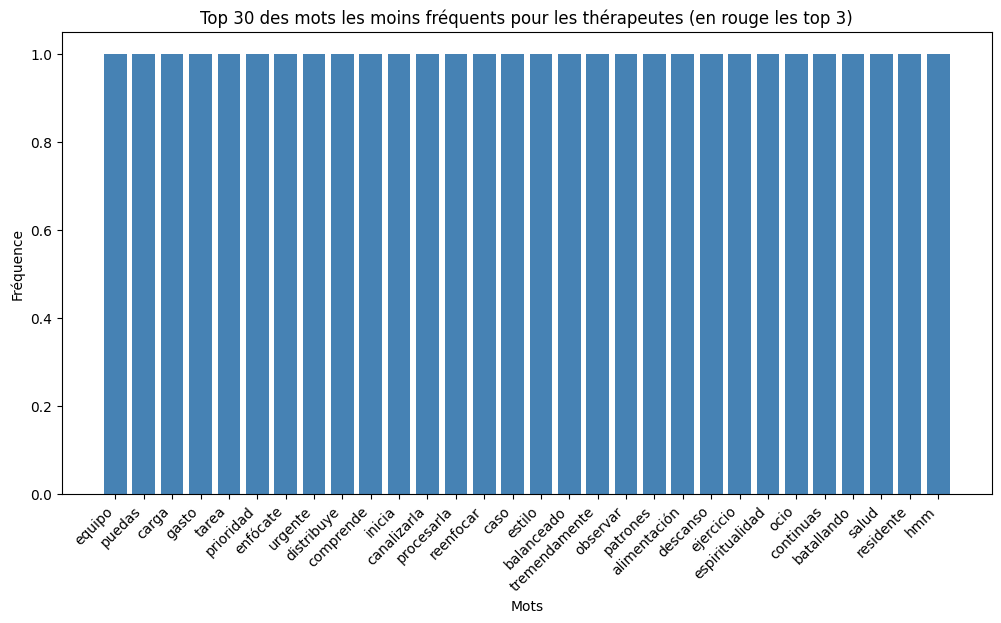
\includegraphics[width=0.80\textwidth]{hist_hapax_therapeute.png}
\caption{Distribution des hapax dans le corpus}
\end{figure}

\clearpage
% ══════════════════════════════════════════════════════════════════════════════
\section{Analyse lexicale — N-grams}

\subsection{Définition}

Un \textbf{n-gram} est une séquence de $n$ mots consécutifs dans un texte. Cette approche
permet de capturer non seulement les mots isolés, mais aussi les associations de mots fréquentes.

\begin{table}[h]
\centering
\begin{tabularx}{\textwidth}{lXX}
\toprule
\textbf{Type} & \textbf{Exemple} & \textbf{Interprétation} \\
\midrule
Unigram (n=1) & \textit{anxiety} (fréq. 342) & Thème dominant \\
Bigram  (n=2) & \textit{mental health} (fréq. 87) & Expression caractéristique \\
Trigram (n=3) & \textit{feel like cry} (fréq. 54) & Patron de détresse \\
\bottomrule
\end{tabularx}
\caption{Exemples de n-grams et leur interprétation}
\end{table}

\subsection{Choix du n optimal}

Il n'existe pas de valeur universelle pour $n$. Deux indicateurs ont été utilisés pour guider
ce choix :

\begin{itemize}
  \item \textbf{Fréquence moyenne} : si elle chute sous un seuil de 5, les n-grams sont trop
        rares pour être statistiquement significatifs.
  \item \textbf{Pourcentage d'hapax} : si plus de 70\,\% des n-grams n'apparaissent qu'une
        seule fois, la taille $n$ est trop grande pour le corpus.
\end{itemize}

L'analyse a montré qu'à partir de $n = 1$, la fréquence diminue déjà fortement. Cependant,
les bigrams et trigrams restent exploitables car le seuil d'hapax n'est pas dépassé.

\subsection{Résultats}

Les bigrams et trigrams apportent un contexte nettement plus riche que les unigrams seuls.
Ils permettront par la suite d'identifier des patrons linguistiques et des thèmes récurrents
pour le topic modeling.

% ══════════════════════════════════════════════════════════════════════════════
\section{Modélisation et extraction de sujets (Topic Modeling)}

Quatre méthodes ont été implémentées et comparées pour identifier les thèmes latents dans
les conversations.

% ── Méthode 1 ─────────────────────────────────────────────────────────────────
\subsection{Méthode 1 — Filtrage par lexique métier}

\subsubsection{Principe}

La première méthode consiste à définir manuellement un dictionnaire où chaque clé est un
thème et chaque valeur est une liste de mots associés à ce thème.

\begin{lstlisting}
lexique = {
    "anxiété":    ["anxiety", "anxious", "worry", "nervous", "panic", "fear", "stress"],
    "dépression": ["depression", "depressed", "sad", "hopeless", "empty", "worthless"],
    "sommeil":    ["sleep", "insomnia", "nightmare", "tired", "fatigue", "wake"],
    "trauma":     ["trauma", "abuse", "ptsd", "flashback", "violent", "assault"],
    "relations":  ["relationship", "family", "friend", "lonely", "isolate", "divorce"],
}
\end{lstlisting}

\subsubsection{Résultats et limites}

L'analyse a révélé que les thérapeutes expriment plus souvent des termes liés aux relations
familiales et amicales que les patients eux-mêmes.

Cependant, cette méthode présente des \textbf{limites importantes} :
\begin{itemize}
  \item Le dictionnaire est subjectif et incomplet : des mots comme \textit{"feeling"} ou
        \textit{"down"} n'appartiennent à aucun thème.
  \item Elle ne tient pas compte du contexte : \textit{"down"} peut relever de l'anxiété ou
        de la dépression selon la phrase.
  \item Elle est statique : elle ne s'adapte pas au vocabulaire réel du corpus.
\end{itemize}

% ── Méthode 2 ─────────────────────────────────────────────────────────────────
\subsection{Méthode 2 — Vectorisation TF-IDF suivie d'un clustering K-Means}

\subsubsection{TF-IDF}

Le \textbf{TF-IDF} (\textit{Term Frequency — Inverse Document Frequency}) est une méthode
de pondération évaluant l'importance d'un mot au sein d'un document par rapport à l'ensemble
du corpus. Il combine deux composantes :

\begin{itemize}
  \item \textbf{Term Frequency (TF)} : fréquence d'un terme dans le document.
  $$tf_{i,j} = \frac{n_{i,j}}{\sum_k n_{k,j}}$$
  où $n_{i,j}$ est le nombre d'occurrences du terme $i$ dans le document $j$.

  \item \textbf{Inverse Document Frequency (IDF)} : pondération par la rareté du mot dans
  le corpus.
  $$idf(w) = \log\!\left(\frac{N}{df_t}\right)$$
  où $N$ est le nombre total de documents et $df_t$ le nombre de documents contenant le terme $t$.
\end{itemize}

Le score final est :
$$w_{i,j} = tf_{i,j} \times \log\!\left(\frac{N}{df_i}\right)$$

Les vecteurs sont ensuite normalisés par la norme L2 afin que la longueur des documents ne
biaise pas les comparaisons.

Grâce au pré-traitement déjà effectué (suppression des stopwords, lemmatisation), l'IDF
discrimine mieux les termes et les scores sont plus significatifs.

\subsubsection{Clustering K-Means}

La méthode du coude (\textit{elbow method}) a été utilisée pour déterminer le nombre optimal
de clusters $K$. L'inertie diminue fortement jusqu'à $K = 6$, puis la courbe se stabilise.
\textbf{$K = 6$ a donc été retenu.}

\subsubsection{Résultats}

\begin{longtable}{p{2.2cm}p{3.8cm}p{3.8cm}p{4cm}}
\toprule
 & \textbf{Patient} & \textbf{Thérapeute} & \textbf{Global} \\
\midrule
\endhead
Cluster 0 & Dépression sévère — idées suicidaires & Soutien initial — écoute & Dépression sévère $\to$ écoute \\
Cluster 1 & Mal-être général — perte de motivation & Accompagnement émotionnel & Mal-être $\to$ accompagnement émotionnel \\
Cluster 2 & Dépression sévère — fatigue mentale & Conseils pratiques & Dépression $\to$ conseils pratiques \\
Cluster 3 & Thérapie de couple — anxiété & Accompagnement en couple & Couple $\to$ thérapie \\
Cluster 4 & Traumatisme — abus — maladie grave & Suivi structuré & Traumatisme $\to$ suivi structuré \\
Cluster 5 & Problèmes familiaux — divorce — identité & Soutien familial & Famille $\to$ soutien familial \\
\bottomrule
\caption{Résultats TF-IDF + K-Means ($K=6$)}
\end{longtable}

Les clusters sont basés sur des similarités lexicales. On note un léger chevauchement entre
les clusters 0 et 2 (dépression), ce qui peut s'interpréter positivement : la dépression peut
provenir de sources différentes (fatigue mentale vs. idées suicidaires). Ce détail révèle que
les conversations ne sont pas aléatoires — les thérapeutes adaptent leur stratégie de réponse
en fonction du type de détresse exprimée par le patient.

% ── Méthode 3 ─────────────────────────────────────────────────────────────────
\subsection{Méthode 3 — Word Embedding (Word2Vec) couplé à K-Means}

\subsubsection{Principe du Word Embedding}

Le \textbf{Word Embedding} (plongement lexical) est une représentation sémantique des mots
sous forme de vecteurs de nombres réels. Deux mots de sens proche ont des vecteurs proches
dans l'espace mathématique.

Contrairement à TF-IDF qui est une \textbf{représentation statistique} (fréquence d'apparition),
Word2Vec est une \textbf{représentation sémantique} : il apprend ce que le mot signifie en
observant les mots qui l'entourent dans le corpus. Ainsi, \textit{"sad"} et \textit{"depressed"}
se trouvent proches dans l'espace vectoriel parce qu'ils apparaissent dans des contextes
similaires.

\subsubsection{Skip-Gram vs CBOW}

Word2Vec propose deux architectures :
\begin{itemize}
  \item \textbf{CBOW} (\textit{Continuous Bag of Words}) : prédit le mot central à partir de
        son contexte. Très rapide sur les grands corpus, mais la moyenne du contexte
        \textit{lisse le bruit}, ce qui peut effacer des nuances importantes.
  \item \textbf{Skip-Gram} (\texttt{sg=1}) : prédit le contexte à partir du mot central.
        Plus adapté aux \textbf{corpus petits et spécialisés} car il génère plus d'exemples
        d'entraînement par mot, compensant le manque de données.
\end{itemize}

\textbf{Skip-Gram a été retenu} pour ce projet, le corpus étant de taille modeste et
spécialisé dans le domaine thérapeutique.

\subsubsection{Paramètres du modèle}

\begin{lstlisting}
model = Word2Vec(
    sentences=all_sentences,
    vector_size=100,   # taille des vecteurs
    window=5,          # contexte de 5 mots de chaque côté
    min_count=3,       # ignore les mots apparaissant moins de 3 fois
    workers=4,
    epochs=10,
    seed=42,
    sg=1               # Skip-Gram
)
\end{lstlisting}

Chaque conversation est vectorisée en calculant la \textbf{moyenne des vecteurs} de ses
tokens présents dans le vocabulaire. Les vecteurs patients et thérapeutes sont ensuite
fusionnés par moyenne pour obtenir un vecteur par échange.

\subsubsection{Résultats}

\begin{longtable}{p{2.2cm}p{3.8cm}p{3.8cm}p{4cm}}
\toprule
 & \textbf{Patient} & \textbf{Thérapeute} & \textbf{Global} \\
\midrule
\endhead
Cluster 0 & Dépression sévère — idées suicidaires & Soutien émotionnel & Dépression $\to$ soutien \\
Cluster 1 & Problèmes sexuels — santé physique & Orientation médicale & Physique $\to$ médical \\
Cluster 2 & Thérapie de couple — anxiété & Accompagnement en couple & Couple $\to$ thérapie \\
Cluster 3 & Mal-être quotidien — divorce & Introspection — gestion émotionnelle & Mal-être $\to$ introspection \\
Cluster 4 & Anxiété — troubles du sommeil & Conseils thérapeutiques & Anxiété $\to$ gestion \\
Cluster 5 & Traumatisme — abus & Accompagnement structuré & Traumatisme $\to$ suivi \\
\bottomrule
\caption{Résultats Word2Vec + K-Means ($K=6$)}
\end{longtable}

Par rapport à TF-IDF, Word2Vec offre une \textbf{meilleure séparation des thèmes}, notamment
pour les patients où la dépression est regroupée dans un seul cluster au lieu de deux. La
cohérence entre les problématiques des patients et les stratégies des thérapeutes est également
plus lisible.

% ── Méthode 4 ─────────────────────────────────────────────────────────────────
\subsection{Méthode 4 — Modèle probabiliste LDA}

\subsubsection{Principe}

Le \textbf{LDA} (\textit{Latent Dirichlet Allocation}) est un modèle génératif probabiliste
permettant de découvrir des sujets latents dans un corpus. C'est une approche bayésienne qui
suppose que chaque document est un \textbf{mélange de thèmes}, et que chaque thème est une
\textbf{distribution de mots}.

Contrairement à K-Means où chaque document appartient à un unique cluster, LDA assigne à
chaque conversation un mélange de thèmes avec des probabilités. Par exemple :

\begin{center}
\textit{"I feel sad and anxious"} $\longrightarrow$ 70\,\% dépression + 30\,\% anxiété
\end{center}

LDA produit deux sorties :
\begin{enumerate}
  \item \textbf{Thèmes $\to$ mots} : distribution des mots caractéristiques pour chaque thème.
  \item \textbf{Documents $\to$ thèmes} : proportion de chaque thème dans chaque conversation.
\end{enumerate}

\subsubsection{Résultats — Patients}

\begin{table}[h]
\centering
\begin{tabularx}{\textwidth}{lXX}
\toprule
\textbf{Topic} & \textbf{Nom suggéré} & \textbf{Mots dominants} \\
\midrule
Topic 0 & Famille — vie quotidienne — anxiété & family, life, anxiety, parent, child \\
Topic 1 & Dépression — addictions — aide & depression, help, substance, hopeless \\
Topic 2 & Relations sociales — pensées & relationship, thought, people, past \\
Topic 3 & Thérapie de couple — anxiété & couple, anxiety, partner, therapist \\
Topic 4 & Sexualité — estime de soi & sexual, esteem, body, love \\
Topic 5 & Relations amoureuses & relationship, boyfriend, trust, person \\
\bottomrule
\end{tabularx}
\caption{Topics LDA — Patients}
\end{table}

\subsubsection{Résultats — Thérapeutes}

\begin{table}[h]
\centering
\begin{tabularx}{\textwidth}{lXX}
\toprule
\textbf{Topic} & \textbf{Nom suggéré} & \textbf{Mots dominants} \\
\midrule
Topic 0 & Suivi thérapeutique & therapist, help, work, session \\
Topic 1 & Parentalité — conseils familiaux & parent, child, family, talk \\
Topic 2 & Relations de couple & relationship, partner, love, work \\
Topic 3 & Bruit résiduel & (mots peu cohérents) \\
Topic 4 & Gestion des pensées — émotions & thought, feeling, way, manage \\
Topic 5 & Dépression — accompagnement & depression, anxiety, help, support \\
\bottomrule
\end{tabularx}
\caption{Topics LDA — Thérapeutes}
\end{table}

\subsubsection{Résultats — Global}

\begin{table}[h]
\centering
\begin{tabularx}{\textwidth}{lXX}
\toprule
\textbf{Topic} & \textbf{Nom suggéré} & \textbf{Mots dominants} \\
\midrule
Topic 0 & Santé / sexualité / aide & health, help, sexual, anxiety \\
Topic 1 & Communication — écoute & talk, people, way, understand \\
Topic 2 & Anxiété — pensées — soutien & anxiety, thought, help, support \\
Topic 3 & Famille — enfants & family, parent, child, live \\
Topic 4 & Thérapie / counseling & therapist, therapy, work, session \\
Topic 5 & Relations de couple & relationship, boyfriend, partner, trust \\
\bottomrule
\end{tabularx}
\caption{Topics LDA — Global}
\end{table}

LDA a permis d'identifier des thématiques principales cohérentes avec le domaine étudié :
relations de couple, parentalité, troubles anxieux et suivi thérapeutique. La flexibilité du
modèle probabiliste permet à chaque conversation d'appartenir à plusieurs thèmes simultanément,
ce qui est plus fidèle à la réalité des échanges thérapeutiques.

% ══════════════════════════════════════════════════════════════════════════════
\section{Comparaison des méthodes}

\begin{table}[h]
\centering
\begin{tabularx}{\textwidth}{lXXX}
\toprule
\textbf{Méthode} & \textbf{Avantages} & \textbf{Inconvénients} & \textbf{Usage} \\
\midrule
TF-IDF + K-Means
  & Simple, rapide, bonne première approche
  & Ignore le sens des mots ; clusters parfois redondants
  & Exploration initiale \\
\midrule
Word2Vec + K-Means
  & Capture les relations sémantiques ; meilleure qualité de clustering ; thèmes plus fins
  & Plus complexe ; résultats moins interprétables directement
  & Regroupement sémantique \\
\midrule
LDA
  & Thèmes interprétables ; modèle probabiliste flexible ; un document peut appartenir à plusieurs thèmes
  & Sensible au pré-traitement ; peut produire du bruit ; choix de $K$ délicat
  & Analyse thématique \\
\midrule
Lexique métier
  & Très simple ; résultats immédiatement lisibles
  & Subjectif, figé, incomplet
  & Introduction / baseline \\
\bottomrule
\end{tabularx}
\caption{Comparaison des quatre méthodes de topic modeling}
\end{table}

\subsection{Conclusion}

Ces méthodes sont \textbf{complémentaires plutôt que concurrentes}.

\begin{itemize}
  \item Le \textbf{LDA} est le plus pertinent pour l'\textbf{analyse thématique} : il produit
        des sujets clairement interprétables et cohérents avec le domaine.
  \item \textbf{Word2Vec} offre la \textbf{meilleure qualité de clustering} en capturant les
        similarités sémantiques.
  \item \textbf{TF-IDF} reste utile comme méthode de référence rapide.
  \item Le \textbf{lexique métier} constitue une bonne introduction mais ses résultats sont
        trop limités pour une analyse approfondie.
\end{itemize}

% ══════════════════════════════════════════════════════════════════════════════
\section{Conclusion générale}

Cette première étape a permis de comprendre la structure du corpus et d'extraire les thèmes
principaux des conversations patient-thérapeute. Le pré-traitement rigoureux (filtrage des
langues, lemmatisation, stopwords) a été déterminant pour la qualité des résultats de topic
modeling.

Les analyses confirment que les conversations ne sont pas aléatoires : les thérapeutes adaptent
leurs stratégies de réponse en fonction des problématiques exprimées par les patients. La
prochaine étape consistera à analyser les sentiments des échanges afin de quantifier la
polarité émotionnelle des conversations.

% ══════════════════════════════════════════════════════════════════════════════
\end{document}